\documentclass{article}

\usepackage[utf8]{inputenc}

\usepackage[sorting=ynt, style=numeric]{biblatex}
\bibliography{references.bib}

\usepackage{graphicx}
\usepackage{subcaption}
\usepackage[section]{placeins}
\usepackage{fullpage}
\usepackage[affil-it]{authblk}
\usepackage{todonotes}

\usepackage{amsmath}
\usepackage{amssymb}
\usepackage{amsthm}
\usepackage{bbold}
\usepackage{mathrsfs}
\usepackage{bm}

\usepackage{algorithm}
\usepackage[noend]{algorithmic} 

\DeclareMathOperator{\Tr}{Tr}
\DeclareMathOperator{\cst}{cst}
\DeclareMathOperator{\Gram}{Gram}
\DeclareMathOperator{\R}{\mathbb{R}}
\DeclareMathOperator{\1}{\mathbb{1}}
\DeclareMathOperator{\E}{\mathbf{E}}
\DeclareMathOperator{\Y}{\mathcal{Y}}
\DeclareMathOperator*{\argmax}{arg\,max}
\DeclareMathOperator*{\argmin}{arg\,min}
\DeclareMathOperator{\dom}{Dom}

\newtheorem{theorem}{Theorem}
\newtheorem{lemma}[theorem]{Lemma}


\title{Non-Uniform Sampling for \\ Stochastic Dual Coordinate Ascent}
\author{R\'emi LE PRIOL}
\affil{Montreal Institute of Learning Algorithms}
\date{\today}

\begin{document}

\maketitle

\section{Introduction}

Non-uniform sampling has been applied to a number fo algorithms to improve their convergence rate. 
They are usually non-adaptive, and transform a dependency in the max of some variables (eg the Lipschitz constant of the gradient of the loss) into  the mean of these variables.
That's the case for SAGA \cite{schmidt2015non}, or SDCA\cite{richtarik}.

Recently some adaptive strategy were proposed, such as \cite{csiba2015stochastic} for SDCA or \cite{osokin2016minding} for BCFW.
\cite{csiba2015stochastic} 's approach was the first adaptive scheme ever proposed and analyzed (at least for sdca), but the analysis gives fairly unpractical results.
Yet it performs well empirically.
Their idea is to sample proportionally to some form of suboptimality, times some Lipschitz factor.
\cite{osokin2016minding} 's strategy is to sample proportionally to the duality gaps of each individual variable. 
As soon as the individual duality gaps are non-uniform enough, they perform significantly better than the uniform scheme.
Their analysis holds only for the sub-linear convergence rate of the classical BCFW though. 

We propose two new sampling scheme for SDCA, and derive according bounds on the convergence rate by mixing ideas from both papers cited above. 
The first scheme samples proportionally to the duality gaps of each individual  variable, so as to spend more time on the worst point so far.
The second scheme is similar to the first one, but it corrects the duality gaps with the Lipschitz constant of the primal problem, so as to spend more time on the points harder to classify.

\section{Theorems}

Denote $h_t = D(\alpha^*) - D(\alpha^{(t)}$ the dual sub-optimality at step t. We can get almost the same bound for the duality gap.

\begin{theorem}[Uniform sampling \cite{shalev-shwartz_accelerated_2013-1}]
	\label{uniform}
	Linear convergence bound with a dependency on the max of the Lipschitz constant.
	\begin{equation}
		h_t \leq (1-\frac{s}{n})^t  h_0
	\end{equation}
	where $ s = \frac{n}{n+R/(\lambda \gamma)} $ is the fixed step-size used in the proof. 
\end{theorem}

We want the linear coefficient $\frac{s}{n}$ to be as large as possible. 
R is an upper bound on the adequate operator norm of the features matrix.
For log-likelihood, $R = \max_{i,y} \| \psi_i(y) \|_2^2 $ is the squared radius of the features. $R/\gamma$ is the smoothness constant of the primal data fitting.
Note that $R/gamma$ is a Lipschitz constant for all the primal loss. $1+R/(n \lambda \gamma)$ is almost a condition number for the primal objective.

\begin{theorem}[Importance Sampling \cite{richtarik}] 
	\label{importance}
	Improved linear convergence bound thanks to larger step sizes. The dependency is now on the mean of the Lipschitz constant.
\end{theorem}

\begin{theorem}[Csiba]
	\label{csiba}
	Should I put Csiba or not? It's quite complicated to explain.
\end{theorem}

\begin{theorem}[Gap sampling (this paper)]
	\label{gap}
	I have a similar improvement as in \cite{osokin2016minding} but with a simpler constant and in the linear coefficient. 
	\begin{equation}
		h_t \leq (1-\frac{s \theta^2}{n})^t  h_0
	\end{equation}
	where $\theta \in [1,\sqrt n] $ is a lower bound on the non-uniformity of the duality gaps.  For a uniform variable, $\theta = 2 / \sqrt 3 $.
\end{theorem}

\begin{theorem}[Gap importance sampling (this paper)]
	\label{gap+}
	I get back the dependency on the mean of the Lipschitz constants, but I lose a bit of the advantage I gained with the gap-sampling.
	\begin{equation}
		h_t \leq (1-\frac{\bar s \theta}{n})^t  h_0
	\end{equation}
\end{theorem}


\section{Proofs}

\paragraph{Setting:} The loss $\phi$ is $1/\gamma$-smooth with respect to $\|.\|_P$.
The regularization $g$ is 1-strongly convex with respect to $\|.\|_{P'}$.
D and D' stand for the dual norms of P and P' respectively. 

\paragraph{One sample descent:} At iteration t, if we sample i, we can lower bound the resulting dual improvement with a line search by considering any step-size $s_i$.
\begin{equation}
	\label{one point descent}
	n (D(\alpha^+) - D(\alpha)) \geq s_i \underbrace{ \big [ \phi(-A_i^Tw) + \phi^*(\alpha_i) + w^T A_i \alpha_i \big ] }_{ \textrm{Fenchel gap} =: g_i} + s_i \bigg ( \frac{\gamma(1-s_i)}{2} - \frac{s_i \|A_i\|^2_{D\rightarrow D'} }{2 \lambda n} \bigg ) \underbrace{\| \beta_i - \alpha_i \|^2_D}{:=d_i^2} 
\end{equation}

For the log-likelihood setting, we pick P the $l^\infty$-norm, D the $l^1$-norm, P' and D' the $l^2$-norm. 
The entropy is 1-strongly convex with respect to the $l^1$ norm so $\gamma = 1$.
We recall that the individual duality gaps can be written $g_i = D(\alpha_i || \beta_i)$.
We define the squared radius of the features for a given sample i as  the maximum $l^2$-norm of the corrected features, which are the columns of the matrix $A_i$.
\begin{equation}
	R_i := \|A_i\|^2_{D\rightarrow D'} = \|A_i\|^2_{1\rightarrow 2} = \max_y \| \psi_i(y)\|_2^2
\end{equation} 
We also define the maximum squared radius as $R=\max_i R_i$.

We obtain the real descent lemma as a lower bound on the expectation of the dual improvement by summing up the inequalities~\eqref{one point descent} with the weights $p_i$ of the sampling probability.

\begin{lemma}[General descent lemma]
	\begin{equation}
		n \mathbb E_p[D(\alpha^+) - D(\alpha)] 
		\geq \underbrace{ \sum_i p_i s_i g_i }_{ \textrm{not the duality gap}} 
		+ \frac{\gamma}{2} \sum_i p_i s_i \bigg ( 1 - s_i \big (1 + \frac{R_i}{\gamma \lambda n} \big ) \bigg ) d_i^2
	\end{equation}
\end{lemma}

\begin{proof}[Proof of Theorem \ref{uniform}]
In the original proof of \cite{shalev-shwartz_accelerated_2013-1}, we set $p_i=1/n$ and $s_i = s = \frac{n}{n+R/(\lambda \gamma)}$. This step size guarantees that the right hand term is positive, leaving us with the inequality:
\begin{equation}
	\mathbb E_p[D(\alpha^+) - D(\alpha)] 
	\geq \frac{s}{n} (P(w) - D(\alpha))
\end{equation}
This inequality gives the final convergence result with the linear constant $s/n = (n+R/(\lambda \gamma))^{-1}$.
\end{proof}


\begin{proof}[Proof of Theorem \ref{importance}]
	\cite{richtarik}
\end{proof}

\begin{proof}[Proof of Theorem \ref{csiba}]
To make the duality gap appear in this formula for arbitrary probability $p$, \cite{csiba2015stochastic} use $p_i s_i = \theta$ constant, whenever $g_i > 0$. 
If the individual duality gap is null $g_i=0$, then they set $p_i=s_i=0$.
\begin{equation}
	n \mathbb E_p[D(\alpha^+) - D(\alpha)] - \theta \underbrace{ \big [ P(w) - D(\alpha) \big ] }_{ \textrm{duality gap}} 
	\geq \theta \frac{\gamma}{2} \sum_i  d_i^2\bigg ( 1 -  \frac{\theta}{p_i} \big ( 1 - \frac{R_i^2}{\gamma \lambda n} \big ) \bigg )
\end{equation}

The negative consequence of that strategy is that he has to enforce $s_i \in [0,1]$ by setting $\theta < \min_i p_i$ where the minimum is taken over the sub-optimal i's (i.e. $p_i>0$).
This a terrible constraint on the step size, as we can't be too non-uniform without taking very small steps.
In effect, it reduces the linear convergence constant $\theta /n$.

Finally, they try to maximize $\theta$ while keeping the right hand side positive.
The is a hard problem on $\theta$ and $p$.
They  solve it only under some restrictions.
\end{proof}

We have a totally different approach that will use among other things the non-uniformity of the Lipschitz constants and the duality gaps.

\begin{proof}[Proof of Theorem \ref{gap}]
	We set $p_i= \frac{g_i}{n(P(w)-D(\alpha))}$. The ascent lemma becomes:
	\begin{equation}
		n \mathbb E_p[D(\alpha^+) - D(\alpha)] 
		\geq \frac{ \frac{1}{n}\sum_i s_i g_i^2 
		+ \frac{\gamma}{2 n}  \sum_i s_i  g_i d_i^2 \ 
		\bigg ( 1 - s_i (1 + \frac{R_i}{\gamma \lambda n}) \bigg ) }{P(w) - D(\alpha)}
	\end{equation}
	We set the same step-size as in the original proof:  
	\begin{equation}
		s_i = s = \frac{n}{n+R/(\lambda \gamma)}	
	\end{equation} 
	We thus have the guarantee that the right hand term is positive. The lemma simplifies in:
	\begin{equation}
		n \mathbb E_p[D(\alpha^+) - D(\alpha)] 
		\geq s \frac{\mathbb E[g_i^2]}{\mathbb E[g_i]} 
		\geq s \mathbb E[g_i] + s \frac{Var(g_i)}{\mathbb E[g_i]}
	\end{equation}
	We find almost the same ascent guarantee as in the uniform case. 
	There's a new positive term on the right, the variance of the gaps divided by their expectation. 
	This is a measure of non-uniformity somehow. 
	If the gaps are all the same, there is indeed no improvement, but if the variance is high, we can expect large gains. 
	We want to improve the constant in the linear convergence guarantee. 
	Let's introduce the non-uniformity of the duality gaps 
	\begin{equation}
		\chi^2(g) := \frac{\mathbb E[g_i^2]}{\mathbb E[g_i]^2 } \in [1,n]
	\end{equation}
	Let's assume that $\chi = \min_t \chi(g^{(t)}) >0$. Now we can write the descent lemma in the same form as in the original proof, but a new constant:
	\begin{equation}
		\mathbb E_p[D(\alpha^+) - D(\alpha)] 
		\geq \frac{s \chi^2}{n} (P(w) - D(\alpha))
	\end{equation}
	So we improved the linear constant by a factor $\chi^2 \ in [1, n]$.	
	To give an idea, if the duality gaps are distributed uniformly on the segment $[u/k,u]$, with k some large number, then $\chi^2= 1 + \frac{1}{3}(1 - \frac{4}{k})$. 
	So when the duality gaps are very evenly distributed between 0 and 1, we can hope an acceleration by a factor $4/3$.
	This is significant enough as it means that we have to spend only $3/4$ of the time to get the desired accuracy, compared to uniform sampling. 
	To get higher values of the non-uniformity, some duality gaps should remain very high while the rest drops close to 0, in a Bernoulli fashion. 
	We did not observe this behaviour, and $4/3$ seems to be a reasonable estimate of what we can get. 
\end{proof}

\begin{proof}[Proof of Theorem \ref{gap+}]
	We set $p_i \propto g_i c_i$ where $c_i = 1+ R/(n \lambda \gamma)$. 
	\begin{equation}
		n \mathbb E_p[D(\alpha^+) - D(\alpha)] 
		\geq \frac{ \sum_i s_i g_i^2 c_i}{\sum_i g_i c_i}  
		+ \frac{ \frac{\gamma}{2}  \sum_i s_i  g_i c_i d_i^2 \ 
		\big ( 1 - s_i c_i \big) }{\sum_i g_i c_i}
	\end{equation}
	Similar to the proof of importance sampling we can now set $s_i= 1/c_i \leq 1$ instead of $s_i=s=1/\max_i c_i$.
	The right hand term is then positive for sure.
	We can take longer steps if the individual Lipschitz constant is high !
	\begin{equation}
		n \mathbb E_p[D(\alpha^+) - D(\alpha)] 
		\geq \frac{ \sum_i g_i^2 }{\sum_i g_i c_i}  
	\end{equation}
	We now use Cauchy-Schwartz :
	 \begin{equation}
		n \mathbb E_p[D(\alpha^+) - D(\alpha)] 
		\geq \frac{ \|g\|_2 }{\|c\|_2} = \frac{ \sqrt{n \E [g^2] } }{\|c\|_2} = \frac{ \sqrt{n} \chi(g) \E [g]}{\|c\|_2}
	\end{equation}
	\begin{equation}
		\mathbb E_p[D(\alpha^+) - D(\alpha)] 
		\geq \frac{ \chi(g) }{ \sqrt{n} \|c\|_2} \E [g]
	\end{equation}
	We have again the non-uniformity of the duality gaps, but this time it is not squared, so we lose a bit on this side.
	The question is now, how does $1/(\sqrt n \|c\|_2)$ compare to $s/n = 1/(n \|c\|_\infty) $.
	We know for sure that the former is larger than the later.
	Stating precisely how much will quantify our improvement.
	We would like to have a clear dependency on $\bar R = \E[R_i]$ instead of $R=\max R_i$ though.
\end{proof}

\section{Experimental comparisons}

In our only experiment, importance sampling has the worst performance. 
Gap and gap-importance sampling perform similarly. 
These may be explained by the gross approximate of the radius I used :

\begin{equation}
	R_i \sim \sum_c R_{i,c} = \sum_c \max_{y_c} \psi_{i,c}(y_c)
\end{equation}

TODO : try with a better approximation. With the formula above, I overestimate the complexity of words which have one letter appear often.

\begin{figure}[ht]
	\center
	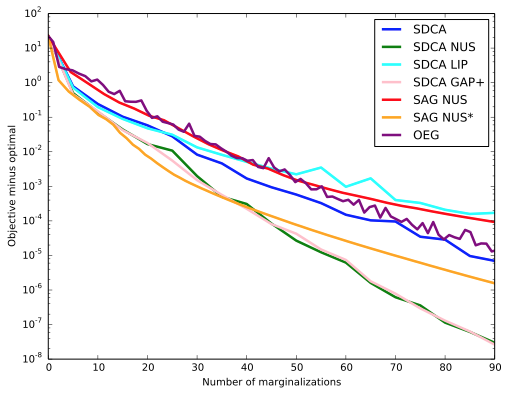
\includegraphics[width=.8\textwidth]{nus1}
	\caption{Comparison of uniform (SDCA), importance (SDCA LIP), gap (SDCA NUS) and gap-importance (SDCA GAP+) schemes on the ocr dataset.}
\end{figure}



\printbibliography

\end{document}
